%!TEX program=xelatex
\documentclass[a4paper,10pt]{article}

\usepackage{amsmath,amssymb}
\usepackage{array}
\usepackage[english]{babel}
\usepackage{csquotes}
\usepackage{ctex}
\usepackage{float}
\usepackage[top=1in,right=1in,bottom=1in,left=1in]{geometry}
\usepackage{hyperref}
\usepackage{indentfirst}
\usepackage{listings}
\usepackage{subcaption}
\usepackage{tcolorbox}
\usepackage{tikz}

\usetikzlibrary{arrows,decorations.pathmorphing,backgrounds,positioning,fit,mindmap,petri}

\hypersetup{
    colorlinks=true,
    linkcolor=blue,
    filecolor=magenta,      
    urlcolor=cyan,
}
\urlstyle{same}

\title{Overview}
\author{Sammy}
\date{\today}

\begin{document}
\maketitle

Monero is a project consists of several components as follows, \par
\begin{minipage}{\linewidth}
	\centering
	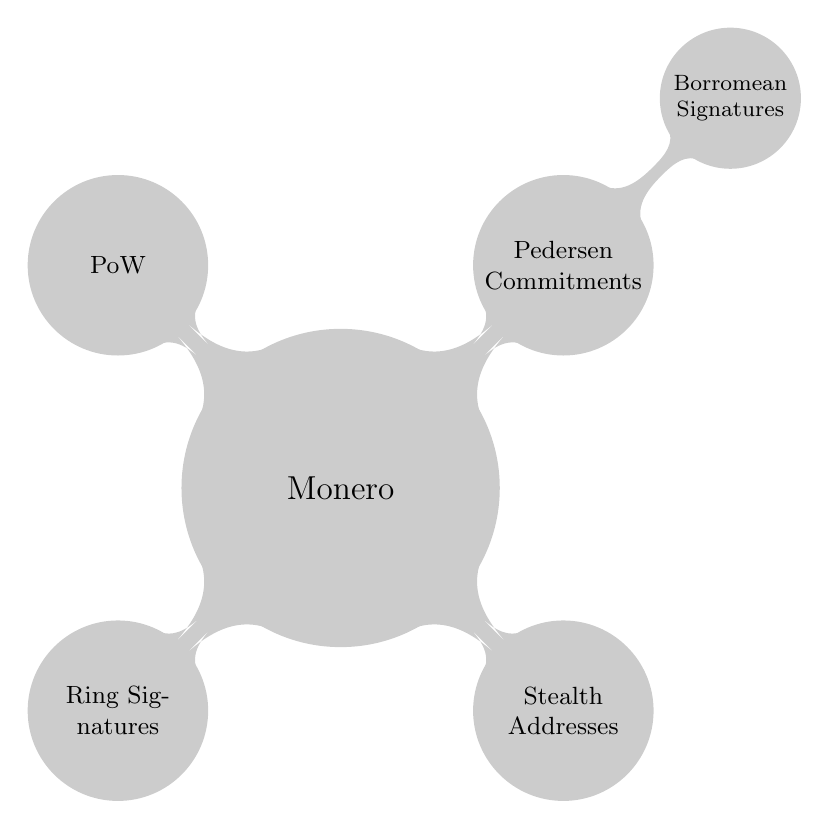
\begin{tikzpicture}[mindmap,every node/.style=concept,concept color=black!20,
			grow cyclic,
			level 1/.append style={level distance=4cm,sibling angle=90},
			level 2/.append style={level distance=3cm,sibling angle=45}]

			\node [root concept] {Monero}
				child {node {Ring Signatures}}
				child {node {Stealth Addresses}}
				child {node {Pedersen Commitments}
					child {node {Borromean Signatures}}
				}
				child {node {PoW}};
	\end{tikzpicture}
\end{minipage}
roles of which are respectively,
	\begin{itemize}
		\item PoW
		\item Pedersen Commitments: amount obfuscation
			\begin{itemize}
				\item \href{./borromean-signatures.pdf}{Borromean Signatures}: space saving
			\end{itemize}
		\item Stealth Addresses: recipient privacy
		\item Ring Signatures: sender privacy
	\end{itemize}


\ifx\ManualOff\undefined
\end{document}
